\documentclass[conference]{IEEEtran}
\IEEEoverridecommandlockouts
\usepackage{iftex}
\ifPDFTeX
  \usepackage[T1]{fontenc}
  \usepackage{newtxtext,newtxmath}
\else
  \usepackage{fontspec}
  \setmainfont{Times New Roman}
\fi
\usepackage{amsmath,amssymb,booktabs,array,graphicx}
\usepackage{placeins}
\setcounter{dbltopnumber}{3}
\renewcommand{\dbltopfraction}{0.95}
\graphicspath{{manuscript/figures/}{figures/}}
\usepackage{xcolor}
\usepackage[hidelinks]{hyperref}
\newcommand{\pending}{\textcolor{red!65!black}{Pending}}
\newcommand{\groot}{GR00T N1.7}
\newcommand{\qwen}{Qwen3-VL-2B}
\title{From Stock to Robot-Adapted VLM Backbones: A Frozen-Feature Study on ALOHA and LIBERO-Goal}
\author{\IEEEauthorblockN{Sittipon Kumda\IEEEauthorrefmark{1} and Rachata Pratheep Na Thalang\IEEEauthorrefmark{1}}\IEEEauthorblockA{King Mongkut's Institute of Technology Ladkrabang\\Thailand\\sittiponkumda@gmail.com, pratheepg49@gmail.com}\thanks{\IEEEauthorrefmark{1}These authors contributed equally to this work.}}
\IEEEpubid{\makebox[\columnwidth][l]{\footnotesize 979-8-3195-1044-0/26/\$31.00~\copyright2026 IEEE}\hspace{\columnsep}\makebox[\columnwidth]{}}
\begin{document}
\raggedbottom
\maketitle
\begin{abstract}
We test whether frozen features from a robot-adapted vision--language
backbone help a newly trained action policy compared with its stock lineage
origin. We read Qwen3-VL-2B and the GR00T N1.7 vision--language subtree at
language layer 16 and independently train the same action-head architecture
within each benchmark. Across three training seeds, GR00T achieves 52.2\%
mean success on ALOHA Transfer Cube, compared with Qwen's 28.7\%, and leads
in every seed pair. On two-camera LIBERO-Goal, both average 89.8\%, with
mixed seed-level differences. Behavioral analysis locates the ALOHA advantage
in completion after an intermediate contact stage; Qwen also reaches that
stage later on selected matched starts where only GR00T succeeds. Two
selected familiar LIBERO goals show opposing advantages: Qwen leads on
wine-to-rack, while GR00T leads or ties on cheese-to-bowl. Both systems
respond to familiar goal changes. Validation flow loss does not reliably
rank development rollout success in these runs. The study evaluates frozen
features through downstream control; the behavioral and prediction probes
identify where the resulting policies differ, without establishing which
representation changes cause those differences.
\end{abstract}
\begin{IEEEkeywords}
vision--language--action, robot learning, frozen representations, evaluation,
imitation learning
\end{IEEEkeywords}

\section{Introduction}
Vision--language--action policies connect visual and language representations
to robot control~\cite{openvla,pi0,grootn1}. When training a new action head,
does a robot-adapted vision--language model (VLM) provide more useful frozen
features than its stock origin? We compare \qwen{} with the vision--language
subtree of \groot{} using the same head design within each benchmark. The released endpoints differ in their training history~\cite{groot17}.

We compare three independently trained heads per backbone. ALOHA Transfer
Cube tests visually guided bimanual transfer with a fixed instruction~\cite{aloha};
LIBERO-Goal tests instruction-conditioned single-arm goals~\cite{libero}.
We evaluate frozen-feature usefulness through closed-loop success with
matched head architectures. Behavioral and prediction probes then locate
differences between the resulting policies. The contributions are a
three-seed endpoint comparison, an analysis of task stages and familiar-goal
responses, and a comparison of validation loss with development success.




\IEEEpubidadjcol
\section{Related Work}
Integrated VLA policies~\cite{openvla,pi0,grootn1} and component studies
such as RoboVLMs~\cite{robovlms} motivate our controlled frozen-feature
comparison. Hand views can
affect manipulation~\cite{handview}; our LIBERO heads receive agent and wrist
views. Critical Interval MSE~\cite{cimse} and LIBERO-PRO~\cite{liberopro}
motivate examining offline validation and evaluation conditions, respectively.

\section{Experimental Design}
\subsection{Backbones and action heads}
We compare frozen \qwen{} and the vision--language subtree of \groot{}.
We cache image and text features at language layer 16. For GR00T this is the
retained final layer; for Qwen it is an intermediate layer followed by its
final RMS normalization. Within each benchmark, processor settings, view
order, token padding, and read depth are matched. Masked padding is removed
before real tokens are right-padded to a fixed budget.

Each backbone feeds a separately trained token adapter and DiT-style action
decoder~\cite{dit}. The decoder learns flow matching~\cite{flow} from
demonstrated actions $a$, noise $\epsilon$, and $t\sim\mathcal U(0,1)$:
\begin{equation}
 \mathcal L=\mathbb E\left[\left\|v_\theta((1-t)\epsilon+ta,t,c)
                    -(a-\epsilon)\right\|_2^2\right].
\end{equation}
Heads have the same design within a benchmark. ALOHA uses 14.0 million
trainable parameters and normalized joint targets; LIBERO uses 19.2 million
and raw end-effector actions. Both predict 16 actions, execute eight, and use
three inference integration steps before replanning. Their decoder widths are
256 and 320, respectively.

% Start the training protocol on page 2.
\newpage
\subsection{Tasks and training}
ALOHA Transfer Cube uses a top camera, robot state, and a fixed instruction
to control two arms. LIBERO-Goal uses agent and wrist cameras, state, and
instructions for ten single-arm goals. ALOHA tests visually guided transfer;
LIBERO tests responses to familiar goals. These benchmarks differ in more
than language or vision alone.

Both backbones use the same episode split within each benchmark. With split
seed 42, ALOHA has 45 training and five validation demonstrations; LIBERO has
450 and 50, with ten percent held out per task. ALOHA normalization uses
training data only. We independently train heads with seeds 3, 4, and 5 to
epoch 250 for ALOHA and epoch 120 for LIBERO. The configuration specifies
highest development success with earliest-epoch tie breaking; the final-test
records evaluate endpoint checkpoints. Saved anchor probes use 50 ALOHA or
100 LIBERO development episodes per head. Validation flow loss uses fixed
RNG seed 4242. Overlapping validation chunks are not independent episodes,
and loss magnitudes are not comparable across the two action spaces.

\subsection{Evaluation}
Each ALOHA head is tested on 200 held-out resets; each LIBERO head is tested
on 40 resets per task (400 total). These resets are separate from development
probes. Within a training-seed pair, the backbones receive matched starts and
policy-sampling seeds. We report per-seed success and 95\% paired-start
percentile bootstrap intervals from 20,000 resamples, stratified by task for
LIBERO. The intervals are conditional on the trained heads; the three training
seeds, not the rollouts, are the independent training replicates.

To examine goal response, we run each policy from 40 matched starts in each
of two scenes with the original and another familiar instruction. The 480
swapped episodes are separate diagnostics. For ALOHA action probes, we replay
saved paths with reset, state, and reward checks and query both native systems
on the same observations with aligned sampling noise. We also continue two
selected Qwen timeouts beyond the original limit. A separate LIBERO audit
repeats 18 selected starts for both backbones, twice per head/start (72
episodes), including two previously discrepant starts. These diagnostics do
not change the locked final tests.

\section{Progression Results}
\subsection{Backbone comparison across training seeds}
Table~\ref{tab:progression} reports the primary held-out progression tests.

\begin{table*}[t]
\centering\small\setlength{\tabcolsep}{5pt}
\caption{Primary progression final tests. Rates are per trained head. $\Delta$
is GR00T minus Qwen in percentage points with a 95\% paired-start bootstrap
interval conditional on the trained pair. G-only/Q-only counts are matched
starts where only that backbone succeeds.}
\label{tab:progression}
\begin{tabular*}{.94\textwidth}{@{\extracolsep{\fill}}llrrrc@{}}\toprule
Benchmark ($n$/head) & Seed & GR00T & Qwen & $\Delta$ (95\% interval) & G-only / Q-only\\\midrule
ALOHA (200) & 3 & 49.5\% & 34.5\% & $+15.0$ ($[7.5,22.5]$) & 47 / 17\\
 & 4 & 42.5\% & 18.0\% & $+24.5$ ($[17.0,32.0]$) & 60 / 11\\
 & 5 & 64.5\% & 33.5\% & $+31.0$ ($[22.5,39.5]$) & 78 / 16\\
LIBERO-Goal (400) & 3 & 89.0\% & 89.8\% & $-0.75$ ($[-4.5,3.0]$) & 30 / 33\\
 & 4 & 88.8\% & 91.8\% & $-3.0$ ($[-6.5,0.5]$) & 22 / 34\\
 & 5 & 91.8\% & 88.0\% & $+3.75$ ($[0.0,7.5]$) & 40 / 25\\\bottomrule
\end{tabular*}
\end{table*}
GR00T leads in all three ALOHA seed pairs, with a mean advantage of
23.5 percentage points (sample SD 8.0). In LIBERO the means are both 89.8\%,
and seed differences change direction (Table~\ref{tab:progression}).

Table~\ref{tab:libero-tasks} lists the ten LIBERO tasks for each seed pair.

\begin{table*}[t]
\centering\small\setlength{\tabcolsep}{3pt}
\caption{LIBERO-Goal task success rates (\%): GR00T/Qwen, with 40 matched starts per head. Each seed denotes a separately trained head pair.}
\label{tab:libero-tasks}
\begin{tabular*}{.94\textwidth}{@{\extracolsep{\fill}}clccc@{}}\toprule
Task & Instruction & Seed 3 & Seed 4 & Seed 5 \\\midrule
0 & open the middle drawer of the cabinet & 90.0/100.0 & 87.5/95.0 & 100.0/100.0 \\
1 & put the bowl on the stove & 97.5/100.0 & 100.0/97.5 & 97.5/97.5 \\
2 & put the wine bottle on top of the cabinet & 97.5/100.0 & 97.5/100.0 & 100.0/95.0 \\
3 & open the top drawer and put the bowl inside & 62.5/75.0 & 70.0/70.0 & 87.5/92.5 \\
4 & put the bowl on top of the cabinet & 100.0/100.0 & 100.0/97.5 & 100.0/95.0 \\
5 & push the plate to the front of the stove & 97.5/90.0 & 67.5/95.0 & 90.0/65.0 \\
\textbf{6} & \textbf{put the cream cheese in the bowl} & \textbf{80.0/60.0} & \textbf{90.0/77.5} & \textbf{82.5/62.5} \\
7 & turn on the stove & 97.5/100.0 & 100.0/97.5 & 95.0/95.0 \\
8 & put the bowl on the plate & 90.0/77.5 & 87.5/87.5 & 77.5/82.5 \\
\textbf{9} & \textbf{put the wine bottle on the rack} & \textbf{77.5/95.0} & \textbf{87.5/100.0} & \textbf{87.5/95.0} \\
\bottomrule
\end{tabular*}
\end{table*}

\subsection{Where do outcomes differ?}
\begin{figure*}[!t]
\centering
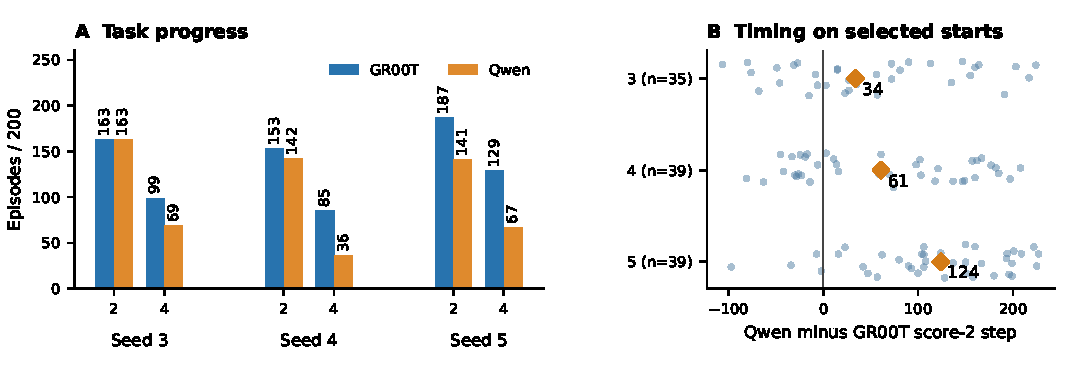
\includegraphics[width=\textwidth]{aloha_progress_timing.pdf}
\caption{ALOHA progress and timing. (A) Score 2: right-finger contact with the cube off the table; score 4: successful handoff. (B) Matched starts where both reached score 2 and only GR00T succeeded. Dots are starts; diamonds are median Qwen-minus-GR00T delays. Positive values mean Qwen was later. }
\label{fig:aloha-progress}
\end{figure*}

GR00T completes more handoffs among episodes reaching score 2
(Fig.~\ref{fig:aloha-progress}A). On matched starts where both policies
reached score 2 and only GR00T succeeded, Qwen generally reached that stage
later (Fig.~\ref{fig:aloha-progress}B). Two selected Qwen timeouts succeeded
at steps 489 and 465 when continued beyond the 400-step limit; both native
systems also succeeded from their reconstructed step-400 states under each of
two shared fresh noise seeds.











LIBERO's aggregate tie conceals goal-level differences. In both scene
cohorts, Qwen leads on wine-to-rack in all three seeds, whereas GR00T leads
or ties on cheese-to-bowl (Fig.~\ref{fig:goal-crossover}). These two goals
were selected for closer analysis because their task-level patterns differ;
each point compares 40 matched starts. In the Task 6 scene with the swapped wine-to-rack instruction, 16 GR00T failures and 4 Qwen failures contacted the
rack without satisfying the goal. In the Task 9 scene with the swapped cheese-to-bowl instruction,
GR00T succeeded after 96 of 107 contacts versus Qwen's 86 of 116.

\begin{figure*}[!t]
\centering
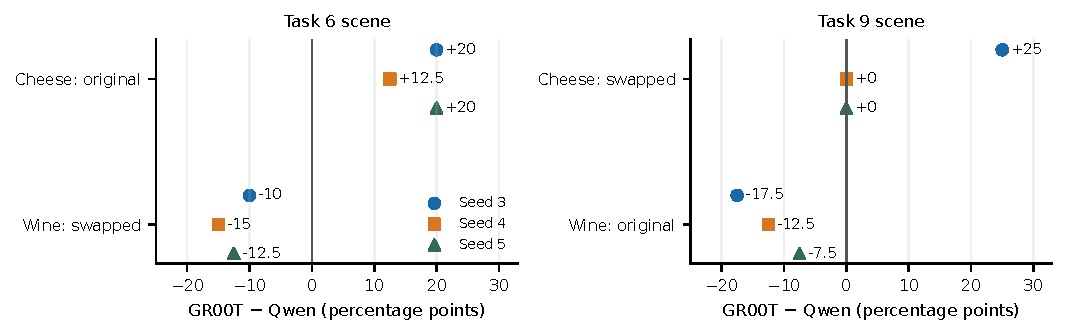
\includegraphics[width=\textwidth]{libero_goal_comparison_review.pdf}
\caption{LIBERO goal comparisons across two scene cohorts. The original task is cheese-to-bowl in Task 6 and wine-to-rack in Task 9; the swapped instruction requests the other goal. Each point is a training-seed pair evaluated on 40 matched starts. Positive differences favor GR00T. }
\label{fig:goal-crossover}
\end{figure*}



\subsection{Instruction response and action clues}
Across 480 episodes with a swapped familiar instruction, neither policy
reached the original goal first. Both systems can redirect to familiar goals,
with both object and destination changed by the request.





On identical initial observations, changing the instruction also changes
layer-16 text features and both heads' predicted first motion commands. In
selected outcome-discordant paths, same-state queries yield different action
chunks near task events, but the magnitude of the difference does not
consistently identify the successful system.

On three selected GR00T-only ALOHA starts, both native systems were queried
at each source path's last replanning boundary before score 2. The predicted gripper targets differ on some observations but not others
(Fig.~\ref{fig:aloha-actions}). All 24 source-policy prefixes across the six selected
discordant starts reproduced archived actions exactly. On four selected reset images, masking the
cube region changed both endpoints' features, adapter contexts, and actions
more than masking an equal-area background patch.





\subsection{Offline loss and development success}
Validation loss reaches its minimum at epoch 25 for all twelve heads and
then rises, while development success often improves (Fig.~\ref{fig:training-progression}). Retrospectively, development success at the minimum-loss
anchor is below the best plotted probe by a median 50 percentage points in
ALOHA and 25.5 points in LIBERO. These best probes need not be eligible for
final checkpoint selection. Within-head Spearman correlations between validation
loss and development success have medians $+0.271$ and $+0.116$. In these runs, validation flow loss alone
does not rank checkpoint rollout success.

\begin{figure*}[!t]
\begin{minipage}[t]{.48\textwidth}
\vspace{0pt}

\centering
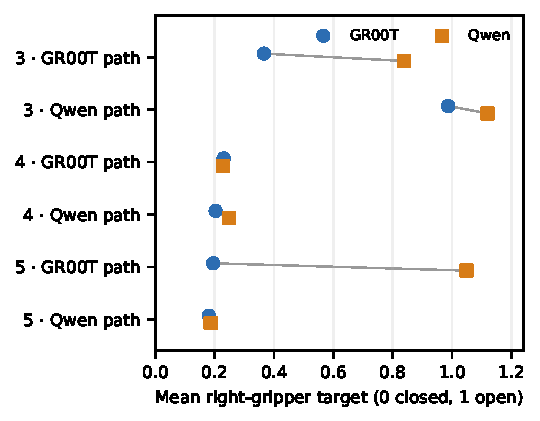
\includegraphics[width=\columnwidth]{aloha_boundary_compact.pdf}
\caption{Predicted right-gripper targets on three selected GR00T-only ALOHA starts. Within each source-path observation, both native systems receive the same image, robot state, and action noise. Markers show mean gripper targets over the next action prefix. Alternative predictions were not executed.}
\label{fig:aloha-actions}
\end{minipage}\hfill
\begin{minipage}[t]{.48\textwidth}
\vspace{0pt}

\centering
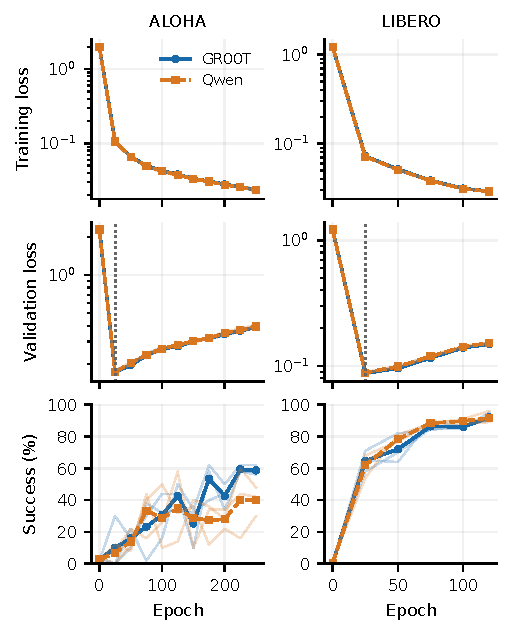
\includegraphics[width=\columnwidth]{training_progression_review.pdf}
\caption{Training and validation flow loss and development success at checkpoint anchors. Loss axes are logarithmic; faint lines are individual heads and bold lines are three-seed means. The dotted line marks epoch 25. Development probes use 50 ALOHA or 100 LIBERO episodes per head and are separate from held-out final tests.}
\label{fig:training-progression}
\end{minipage}
\end{figure*}



\clearpage
\twocolumn
\section{Limitations}
Task-level comparisons and outcome-selected probes are descriptive. The timing
subsets and two extended episodes do not estimate the prevalence or cause of
failures. Alternative action predictions were not executed, and image masking
may produce unfamiliar inputs. These probes do not identify which feature
changes cause better control. The equal LIBERO means do not establish
equivalence, and dependent checkpoint probes do not establish test-set
performance or prove overfitting.

The study compares two frozen endpoints from one lineage. The intervening
Cosmos-Reason2 model~\cite{groot17} is not tested, so the endpoint contrast cannot be
attributed to one pretraining stage. The results concern newly trained heads,
not the complete released GR00T policy. ALOHA and LIBERO differ in task,
embodiment, camera views, action space, and head size; their contrast cannot
isolate a language, vision, or embodiment effect.

The primary comparison uses three independent training seeds per backbone.
Per-seed reporting
shows the observed training variation; paired-start intervals are conditional
on the trained heads. Familiar LIBERO goal swaps do not test unseen language
or tasks.
Phase measures are simulator predicates. Selected same-state probes use
outcome-discordant examples, so they reveal candidate decision points rather
than failure prevalence or causal feature effects. The fixed demonstration
split, including five ALOHA validation episodes, also limits checkpoint
selection coverage.

The LIBERO repeat audit deliberately included two previously discrepant
starts. Among 36 selected head/start pairs, both repeats matched the locked
outcome in 31, disagreed with each other in four, and both differed from the
locked outcome in one; all five were wine-task pairs. All new initial state
and both camera hashes matched across repeats, but the locked records lack a
separate wrist-image hash. At the first action difference above $10^{-6}$ in
10 pairs, state and agent-view hashes matched while wrist-view hashes differed.
Two fixed-action checks showed occasional one-level 8-bit wrist-render
differences with matching simulator states; they do not establish the size
or cause of differences in the original repeat episodes. This selected audit
is not a benchmark-wide reproducibility estimate.

% Begin the conclusion in the next column.
\newpage
\section{Conclusion}
With matched action-head architectures, frozen GR00T features support higher
ALOHA success across all three training seeds, but no aggregate advantage
on LIBERO-Goal. GR00T completes more ALOHA transfers among episodes reaching
score 2; on selected matched starts where only GR00T succeeds, Qwen reaches
that stage later. In LIBERO, the aggregate tie conceals opposing advantages
on the two selected familiar goals. Both systems respond to familiar
instruction changes. These results evaluate the control usefulness of the
frozen features. Timing and action probes locate candidate decision points for further study. Finally, validation flow
loss alone did not reliably rank development rollout success in these runs.

\begin{thebibliography}{12}
\bibitem{openvla} M. J. Kim et al., ``OpenVLA: An open-source vision-language-action
model,'' arXiv:2406.09246, 2024.
\bibitem{pi0} K. Black et al., ``$\pi_0$: A vision-language-action flow model for
general robot control,'' arXiv:2410.24164, 2024.
\bibitem{grootn1} NVIDIA, ``GR00T N1: An open foundation model for generalist
humanoid robots,'' arXiv:2503.14734, 2025.
\bibitem{groot17} NVIDIA, ``GR00T-N1.7-3B,'' released model card and configuration,
\url{https://huggingface.co/nvidia/GR00T-N1.7-3B}, accessed Oct. 21, 2026.
\bibitem{robovlms} X. Li et al., ``What matters in building vision--language--action
models for generalist robots,'' \emph{Nature Machine Intelligence}, vol. 8,
pp. 158--172, 2026, doi: 10.1038/s42256-025-01168-7.
\bibitem{aloha} T. Z. Zhao, V. Kumar, S. Levine, and C. Finn, ``Learning fine-grained
bimanual manipulation with low-cost hardware,'' in \emph{Proc. RSS}, 2023.
\bibitem{libero} B. Liu et al., ``LIBERO: Benchmarking knowledge transfer for
lifelong robot learning,'' in \emph{NeurIPS Datasets and Benchmarks}, 2023.
\bibitem{handview} K. Hsu, M. J. Kim, R. Rafailov, J. Wu, and C. Finn,
``Vision-based manipulators need to also see from their hands,''
in \emph{Proc. ICLR}, 2022.
\bibitem{cimse} H. Huang, T. Zheng, Y. Chen, J. You, and Y. Gao, ``Critical interval
MSE: Toward reliable offline validation for robot manipulation policies,''
arXiv:2606.29898, 2026.
\bibitem{liberopro} X. Zhou, Y. Xu, G. Tie, Y. Chen, G. Zhang, D. Chu, P. Zhou,
and L. Sun, ``LIBERO-PRO: Towards robust and fair evaluation of vision-language-action
models beyond memorization,'' arXiv:2510.03827, 2025.
\bibitem{dit} W. Peebles and S. Xie, ``Scalable diffusion models with transformers,''
in \emph{Proc. ICCV}, 2023.
\bibitem{flow} Y. Lipman, R. T. Q. Chen, H. Ben-Hamu, M. Nickel, and M. Le,
``Flow matching for generative modeling,'' in \emph{Proc. ICLR}, 2023.
\end{thebibliography}
% Fail compilation if this draft grows beyond the conference's six-page limit.
% clearpage flushes the last content page, so the next-page counter is at most 7.
\clearpage
\ifnum\value{page}>7
  \PackageError{camera-ready}{Manuscript exceeds six pages}{Reduce content without changing the conference layout.}
\fi
\end{document}
